Spočítejte:

\begin{enumerate}

	\item  Taylorovu řadu v nule ($a = 0$) polynomu $p(x) = 7x^5 - \frac{4}{7} x^3 + 3\pi x^2 - 42$.

		\solution{
			Nejprve spočítáme derivace:
			\begin{align*}
				p'(x) = \left( 7x^5 - \frac{4}{7} x^3 + 3\pi x^2 - 42 \right)^{(1)} &= 35x^4 - \frac{12}{7}x^2 + 6\pi x \\
				p''(x) = \left( 7x^5 - \frac{4}{7} x^3 + 3\pi x^2 - 42 \right)^{(2)} &= 140x^3 - \frac{24}{7}x + 6\pi  \\
				p'''(x) = \left( 7x^5 - \frac{4}{7} x^3 + 3\pi x^2 - 42 \right)^{(3)} &= 420x^2 - \frac{24}{7}  \\
				p''''(x) = \left( 7x^5 - \frac{4}{7} x^3 + 3\pi x^2 - 42 \right)^{(4)} &= 840x  \\
				p'''''(x) = \left( 7x^5 - \frac{4}{7} x^3 + 3\pi x^2 - 42 \right)^{(5)} &= 840  \\
				p''''''(x) = \left( 7x^5 - \frac{4}{7} x^3 + 3\pi x^2 - 42 \right)^{(k)} &= 0 \tag{pro každé $k \geq 6$}
			\end{align*}

			Z vzorce máme:
			\begin{align*}
				T^{p, 0}(x) &= p(0) + \sum_{n = 1}^\infty \frac{p^{(n)}(0)}{n!} (x-0)^n \\
				&= p(0) + \sum_{n = 1}^\infty \frac{p^{(n)}(0)}{n!} x^n \\
				&= -42 + \frac{0}{1!}x + \frac{6\pi}{2!}x^2 + \frac{-24/7}{3!}x^3 + \frac{0}{4!}x^4 + \frac{840}{5!}x^5 \\
				&= p(x)
			\end{align*}
		}
	
	\item  Taylorovu řadu v jedničce ($a = 1$) funkce $7x^5 - \frac{4}{7} x^3 + 3\pi x^2 - 42$.

		\solution{
			Derivace už máme spočítané.
			Z vzorce máme:
			\begin{align*}
				T^{p, 1}(x) = &p(1) + \sum_{n = 1}^\infty \frac{p^{(n)}(1)}{n!} (x-1)^n \\
				=
					&\left( 7 - \frac{4}{7} + 3\pi -42 \right) + \left(35 - \frac{12}{7} + 6\pi \right) (x-1) \\
					&+ \frac{140 - \frac{24}{7} + 6\pi}{2!}(x-1)^2 + \frac{420 - \frac{24}{7}}{3!}(x-1)^3 \\
					&+ \frac{840}{4!}(x-1)^4 + \frac{840}{5!}(x-1)^5 \\
				= &p(x)
			\end{align*}

			Podívejte se na grafy $p$ a Taylorova polynomu malých stupňů v bodě 0 a 1:
			\begin{itemize}

				\item  Stupně 0: Obrázek~\ref{fig:taylor_0_pol}.
				\item  Stupně 1: Obrázek~\ref{fig:taylor_1_pol}.
				\item  Stupně 2: Obrázek~\ref{fig:taylor_2_pol}.
				\item  Stupně 3: Obrázek~\ref{fig:taylor_3_pol}.
				\item  Stupně 4: Obrázek~\ref{fig:taylor_4_pol}.
				\item  Stupně 5: Obrázek~\ref{fig:taylor_5_pol}.

			\end{itemize}

			\begin{figure}[H]
				\centering
				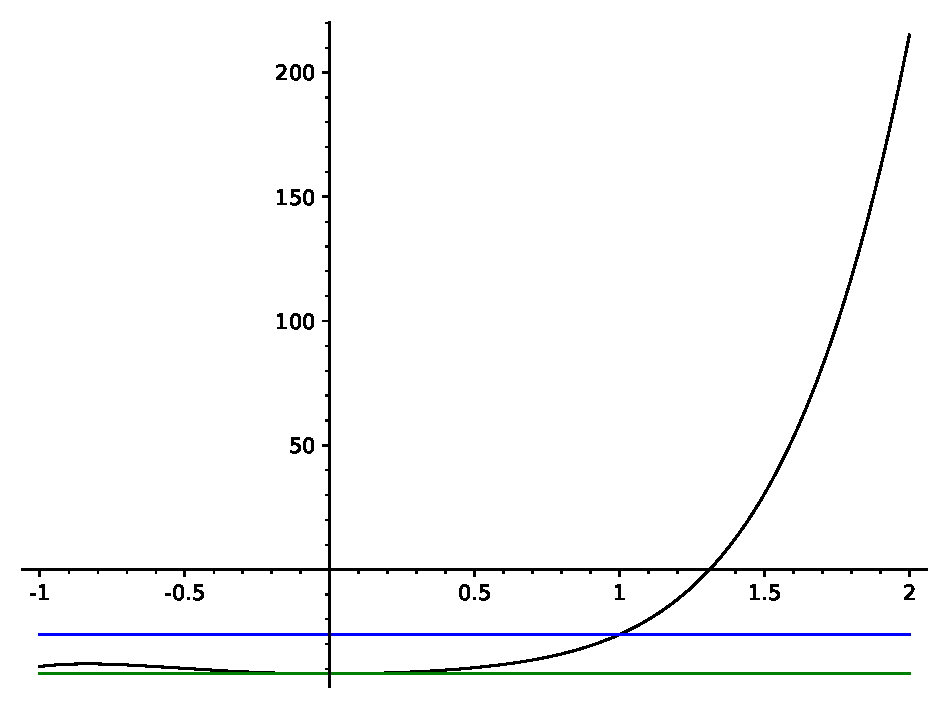
\includegraphics{cviceni_10/fig/taylor_pol_0.pdf}
				\caption{$p(x) = 7x^5 - \frac{4}{7} x^3 + 3\pi x^2 - 42$ černě, $T_0^{p, 0}$ zeleně, $T_0^{p, 1}$ modře.}
				\label{fig:taylor_0_pol}
			\end{figure}

			\begin{figure}[H]
				\centering
				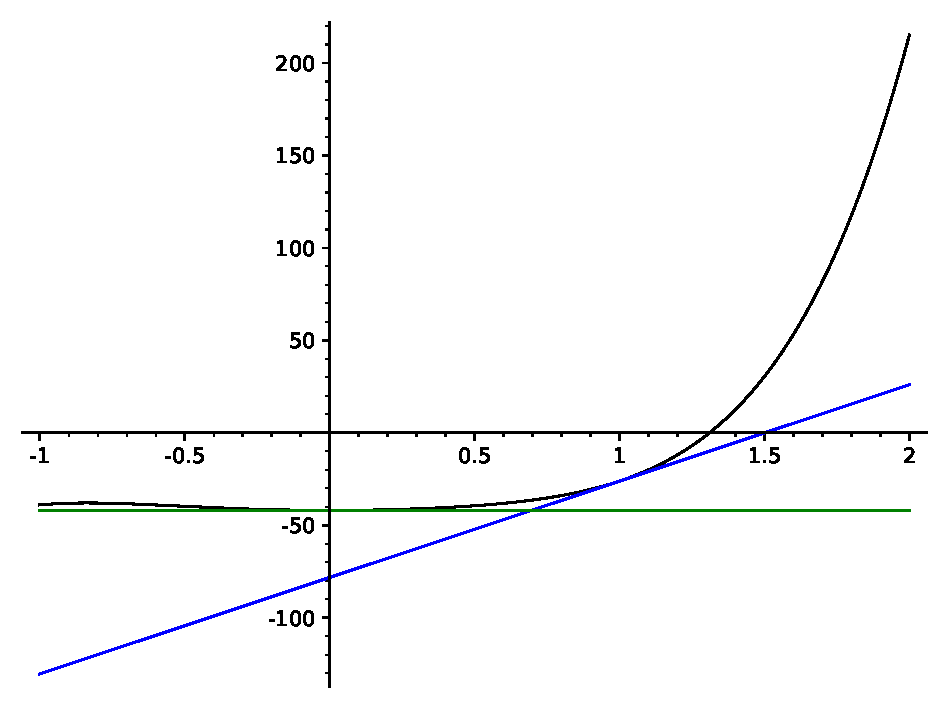
\includegraphics{cviceni_10/fig/taylor_pol_1.pdf}
				\caption{$p(x) = 7x^5 - \frac{4}{7} x^3 + 3\pi x^2 - 42$ černě, $T_1^{p, 0}$ zeleně, $T_1^{p, 1}$ modře.}
				\label{fig:taylor_1_pol}
			\end{figure}

			\begin{figure}[H]
				\centering
				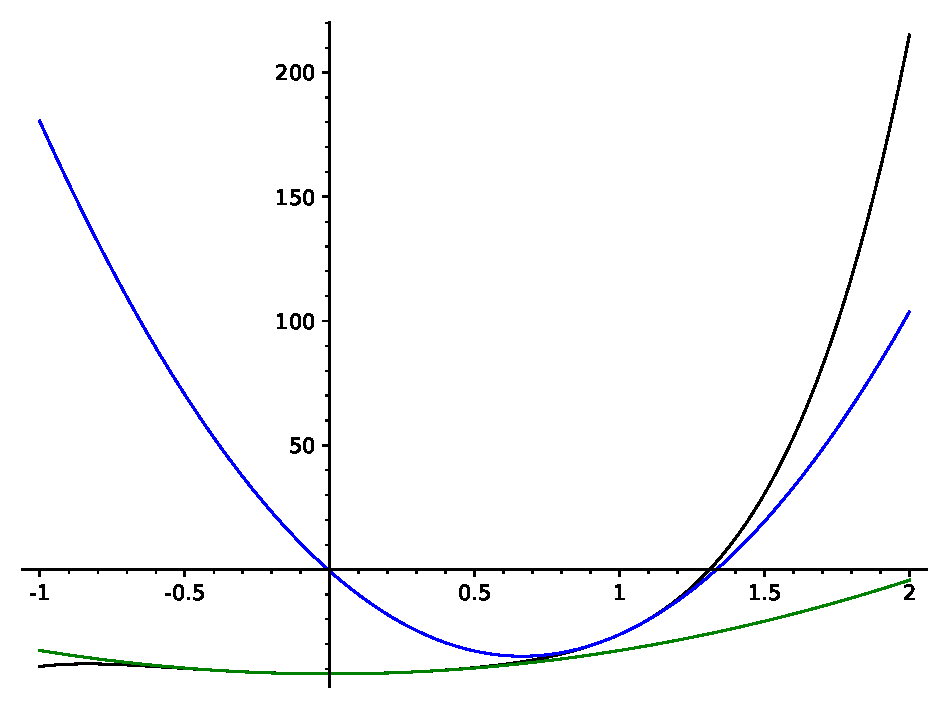
\includegraphics{cviceni_10/fig/taylor_pol_2.pdf}
				\caption{$p(x) = 7x^5 - \frac{4}{7} x^3 + 3\pi x^2 - 42$ černě, $T_2^{p, 0}$ zeleně, $T_2^{p, 1}$ modře.}
				\label{fig:taylor_2_pol}
			\end{figure}

			\begin{figure}[H]
				\centering
				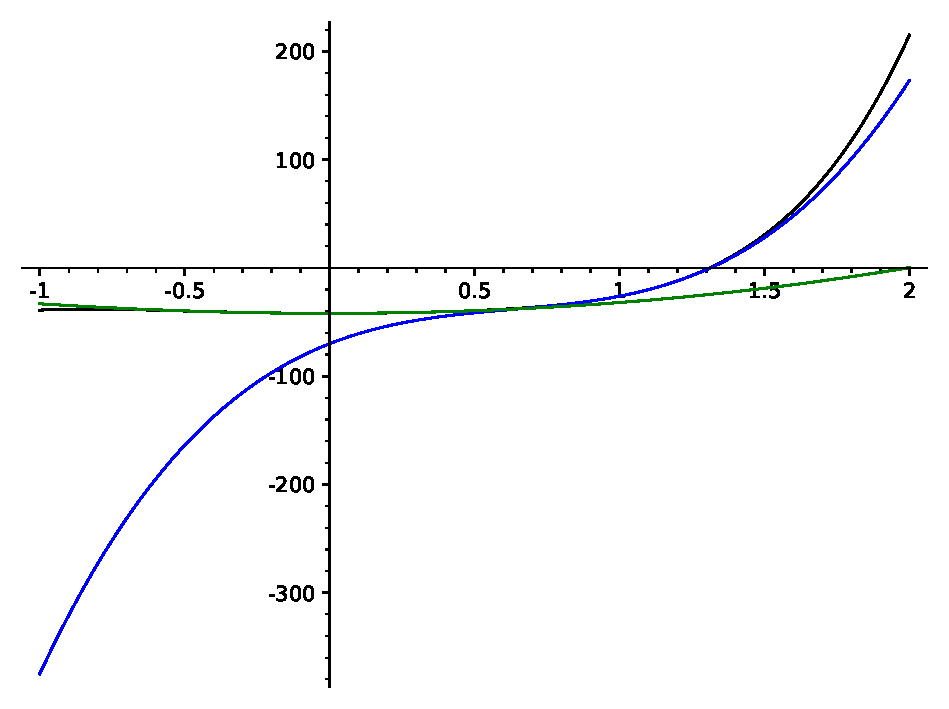
\includegraphics{cviceni_10/fig/taylor_pol_3.pdf}
				\caption{$p(x) = 7x^5 - \frac{4}{7} x^3 + 3\pi x^2 - 42$ černě, $T_3^{p, 0}$ zeleně, $T_3^{p, 1}$ modře.}
				\label{fig:taylor_3_pol}
			\end{figure}

			\begin{figure}[H]
				\centering
				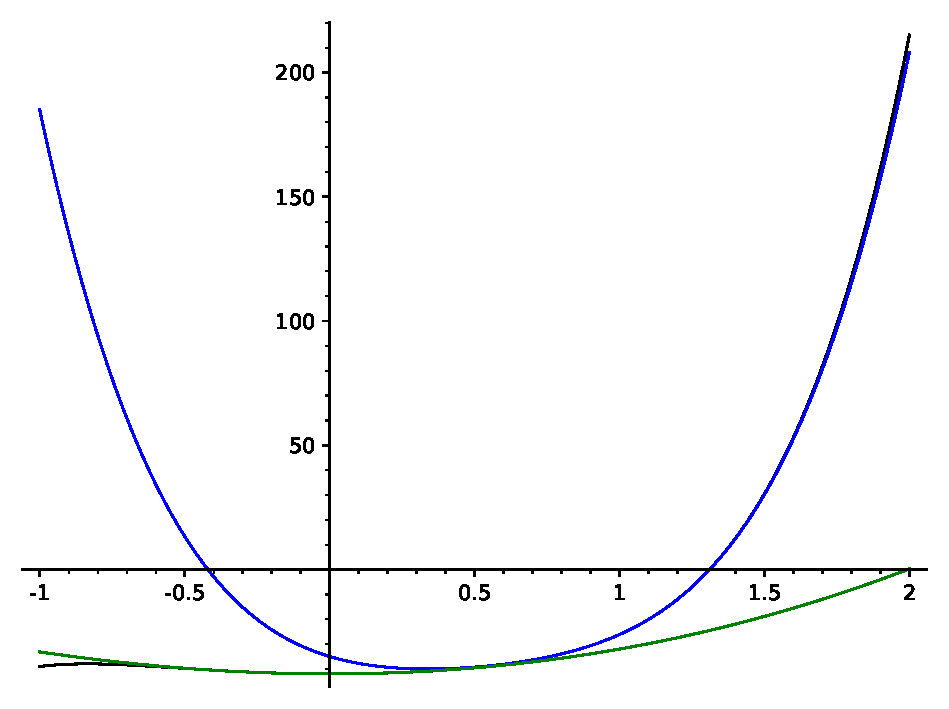
\includegraphics{cviceni_10/fig/taylor_pol_4.pdf}
				\caption{$p(x) = 7x^5 - \frac{4}{7} x^3 + 3\pi x^2 - 42$ černě, $T_4^{p, 0}$ zeleně, $T_4^{p, 1}$ modře.}
				\label{fig:taylor_4_pol}
			\end{figure}

			\begin{figure}[H]
				\centering
				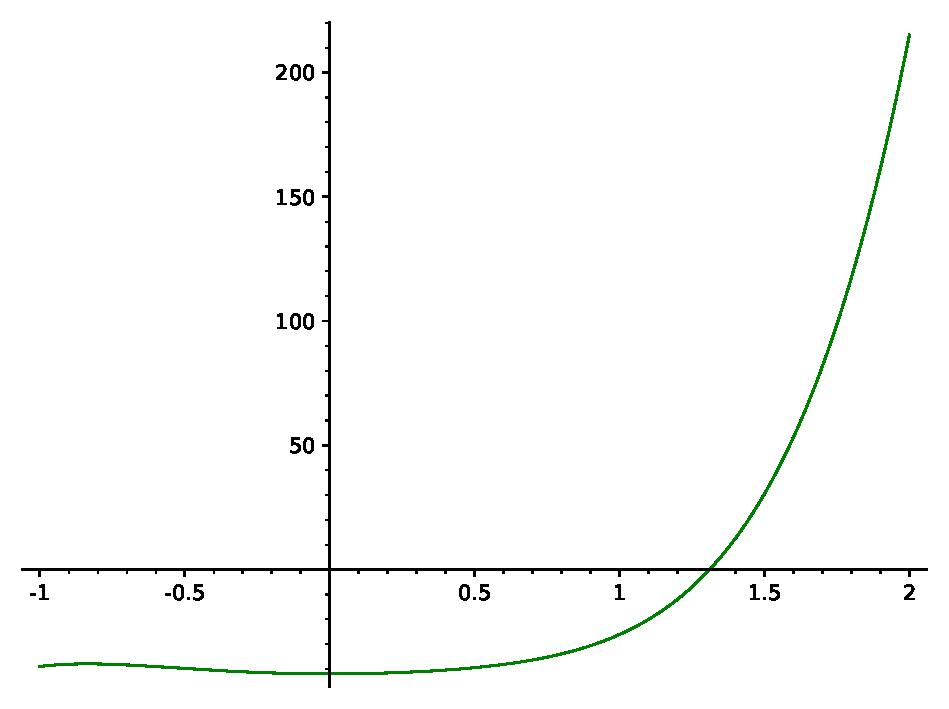
\includegraphics{cviceni_10/fig/taylor_pol_5.pdf}
				\caption{$p(x) = 7x^5 - \frac{4}{7} x^3 + 3\pi x^2 - 42$ černě, $T_5^{p, 0}$ zeleně, $T_5^{p, 1}$ modře.}
				\label{fig:taylor_5_pol}
			\end{figure}
		}

	\item  Taylorovu řadu v nule ($a = 0$) funkce $\ln(1+x)$

		\solution{
			Znova spočítáme prvních pár derivací a zkusíme vykoukat, jak budou vypadat další.
			\begin{align*}
				\ln(1 + x)' &= \frac{1}{1+x} = (1+x)^{-1} \\
				\ln(1 + x)'' &= (-1) \cdot(1+x)^{-2} \\
				\ln(1 + x)''' &= (-2) \cdot (-1) \cdot (1+x)^{-3} \\
				\ln(1 + x)'''' &= (-3) \cdot (-2) \cdot (-1) \cdot (1+x)^{-4} \\
				\ln(1 + x)''''' &= (-4) \cdot (-3) \cdot (-2) \cdot (-1) \cdot (1+x)^{-5}
			\end{align*}

			Matematickou indukcí dokážeme, že $n$-tá derivace má následující tvar:
			$$\left( \ln(1+x) \right)^{(n)} = (-1)^{n+1} (n-1)! (1+x)^{-n}$$

			Taylorova řada v nule tedy má tvar:
			\begin{align*}
				T^{\ln(1+x), 0}(x) &= \ln(1+0) + \sum_{n = 1}^{\infty} \frac{\left( \ln(1+x) \right)^{(n)}(0)}{n!} (x-0)^n \\
				&= 0 + \sum_{n = 1}^{\infty} \frac{\left( \ln(1+x) \right)^{(n)}(0)}{n!} x^n \\
				&= \sum_{n = 1}^{\infty} \frac{(-1)^{n+1}x^n}{n} \\
				&= x - \frac{x^2}{2} + \frac{x^3}{3} - \frac{x^4}{4} + \frac{x^5}{5} - \ldots
			\end{align*}
		}

	\item  Pomocí Taylorova polynomu v nule odhadněte $\sin(0.1)$ s přesností $10^{-6}$ (dostanete hodnotu, která je zaručeně v intervalu plus minus $10^{-6}$ od té skutečné).

		\solution{
			Z minula známe Taylorovu řadu funkce sinus:
			$$\sin(x) = \sum_{k = 0}^{\infty} \frac{(-1)^k x^{1 + 2k}}{(1 + 2k)!} = x - \frac{x^3}{6} + \frac{x^5}{120} - \ldots$$

			Chceme vzít Taylorův polynom stupně $n$ takový že $10^{-6}$ bude větší rovna absolutní hodnotě zbytku:
			$$R_n^{\sin, 0}(x) = \sin(x) - T_{n}^{\sin, 0}(x)$$

			Použijeme Lagrangeův odhad zbytku.
			Sinus je definován a má všechny derivace na intervalu $(a, b) = (0, 0.1)$.
			Pak existuje $c \in (a, b)$ takové, že:
			$$R_n^{\sin, a}(b) = \frac{\sin^{(n+1)}(c)}{(n+1)!} (b-a)^{n+1}$$

			Víme, že $n+1$ tá derivace $\sin x$ je $\pm \sin x$ nebo $\pm cos x$, speciálně pro každé reálné číslo platí $|\pm\sin(x)| \leq 1$ a také $|\pm\cos(x)| \leq 1$.
			Absolutní hodnotu zbytku tedy můžeme odhadnout jako:
			$$|R_n^{\sin, a}(b)| \leq \frac{1}{(n+1)!} (b-a)^{n+1}$$

			Konkrétně:
			$$|R_n^{\sin, 0}(0.1)| \leq \frac{1}{(n+1)!} (0.1)^{n+1}$$
			Pro jednotlivá $n$ snadno spočítáme chybu:
			\begin{align*}
				|R_1^{\sin, 0}(0.1)| &\leq 0.005 \\
				|R_2^{\sin, 0}(0.1)| &\leq 0.0001666666666 \\
				|R_3^{\sin, 0}(0.1)| &\leq 4.16666666 \cdot 10^{-6} \\
				|R_4^{\sin, 0}(0.1)| &\leq 8.33333333 \cdot 10^{-8} < 10^{-6}
			\end{align*}

			Rozmyslete si, že pro $n$-té derivace, kde $n$ je sudé jsme mohli použít lepší odhad
			$$\forall x \in (0, b) \colon |\pm \sin(x)| \leq b.$$
			Ale pro lichá $n$ nám tohle moc nepomůže.

			Rozmyslete si, že speciálně pro sinus stačí vzít první tři členy (protože člen $x^4$ je nulový).
			Tedy $T_3^{\sin, 0}(0.1) \in (\sin(0.1) - 10^{-6},  \sin(0.1) + 10^{-6})$.
		}

	\item  Jak byste odhadovali přesnost Taylorova polynomu v nule pro aproximaci $\ln(1+x)$?

		\solution{
			Potřebujeme odhadnout
			$$| (-1)^{n+1} (n-1)! (1+x)^{-n} | \leq \frac{(n-1)!}{(1+x)^n} \leq (n-1)! $$
			Pomocí Stirlingovy formule si rozmyslete, jestli jsme v poslední nerovnosti nezahodili příliš mnoho.

			Získáváme tedy o poznání horší tvar zbytku.
			$$|R_n^{\ln(1+x), 0}| \leq \frac{1}{n}$$
		}

	\item  Spočítejte Taylorovu řadu pro $\sqrt{1+x}$.

		\solution{
			Zavedeme si užitečné značení (zobecnění binomického čísla) pro $a \in \mathbb{R}, n \in \mathbb{N}$ značíme:
			$$\binom{a}{n} = \prod_{j = 1}^{n} \frac{a - j + 1}{j} = \frac{a \cdot (a-1) \cdot (a-2) \cdot \ldots \cdot (a - (n-1))}{n!}$$
			Bez tohoto zápisu by to šlo taky, ale tohle bude elegantnější zápis.

			Pak spočítáme derivace:
			\begin{align*}
				f'(x) = \left( \sqrt{1+x} \right)^{(1)} &= \frac{1}{2} (1+x)^{-1/2} \\
				f''(x) = \left( \sqrt{1+x} \right)^{(2)} &= \frac{1}{2} \left( \frac{-1}{2} \right) (1+x)^{-3/2} \\
				f'''(x) = \left( \sqrt{1+x} \right)^{(3)} &= \frac{1}{2} \left( \frac{-1}{2} \right) \left( \frac{-3}{2} \right) (1+x)^{-5/2} \\
			\end{align*}

			A dopočítáme že
			$$\sqrt{1+x} = 1 + \binom{1/2}{1} x + \binom{1/2}{2}x^2 + \binom{1/2}{3}x^3 + \ldots$$
		}

\end{enumerate}

